\documentclass[12pt]{article}
\usepackage[utf8]{inputenc}
\usepackage[T1]{fontenc}
%\usepackage{fullpage}
%\usepackage{psfig}
\usepackage{times}
\usepackage{xspace}
\usepackage[hyphens]{url}
\usepackage{geometry}
\usepackage{graphicx}
%\usepackage[tight]{subfigure}
\usepackage{array}
\usepackage{makecell}
\usepackage{multicol}
\usepackage{algorithm}
\usepackage{algorithmic}
\usepackage{amssymb}
\usepackage{amsmath}
\usepackage{amsfonts}
\usepackage{fancyhdr}
\usepackage{booktabs}
\usepackage{listings}
\usepackage{ifthen}
\usepackage{wrapfig}
\usepackage[sort,compress,numbers]{natbib}
\usepackage[compact]{titlesec}
\usepackage[usenames,dvipsnames]{xcolor}
%\usepackage{comment}
\usepackage{xcolor,colortbl}

% \usepackage[hidelinks]{hyperref}
\usepackage{multirow}
\usepackage{framed}
\usepackage{enumitem}
\usepackage[font=footnotesize,font=bf,it]{caption} 
\usepackage{epstopdf} 
%\usepackage{subfig, enumerate}
%\usepackage{subcaption}
\usepackage[FIGBOTCAP,normal,bf,tight]{subfigure}
\usepackage{csquotes}
\usepackage{tabularx}
\usepackage{beramono}
\usepackage{pdfpages}
\usepackage{listings}
\usepackage{mathptmx}	% Use the Postscript Times font

\definecolor{dkgreen}{rgb}{0,0.6,0}
\definecolor{gray}{rgb}{0.5,0.5,0.5}
\definecolor{mauve}{rgb}{0.58,0,0.82}

\PassOptionsToPackage{hyphens}{url}\usepackage[colorlinks=true,urlcolor=blue]{hyperref}

\urlstyle{same}
\usepackage{wrapfig}

\definecolor{dkgreen}{rgb}{0,0.6,0}
\definecolor{gray}{rgb}{0.5,0.5,0.5}
\definecolor{mauve}{rgb}{0.58,0,0.82}

\usepackage{tikz}
\newcommand{\swatch}[1]{\tikz[baseline=-0.6ex] \node[fill=#1,shape=rectangle,draw=black,thick,minimum width=5mm,rounded corners=2pt](){};}

\newcommand{\proptitle}{Sandia Technical Report: Balar: SST/GPGPU-Sim Integration}
\newcommand{\shorttitle}{Balar}

\newcommand{\system}{\shorttitle\xspace}

\geometry{verbose,papersize={8.5in,11in},
		left={1in},right={1in},top={1in},bottom={1in}}
\pagestyle{fancy}
\lhead{Purdue University: \shorttitle}
\rhead{Sandia TR}
\renewcommand{\footrulewidth}{0.4pt}
\lfoot{Purdue University, Sandia National Labs}
\cfoot{}
\rfoot{\thepage}



% \def\IncSpacing{\addtolength{\baselineskip}{0.5\baselineskip}}
% \def\IncSpacing{\addtolength{\baselineskip}{0.22\baselineskip}}
% \def\DecSpacing{\addtolength{\baselineskip}{-0.33333\baselineskip}}

%\newfont{\cour}{cmtt10}

%\renewcommand{\paragraph}[1]{\medskip\noindent\textbf{#1.}}
% \renewcommand{\paragraph}[1]{\smallskip\noindent\textbf{#1.}}

% \setlength{\itemsep}{20pt}
\addtolength{\itemsep}{-1in}
% Reduce spacing in lists
\setlist[itemize]{noitemsep} % noitemsep -> nosep will make it even more compact, but not advisable
\setlist[enumerate]{noitemsep}
\setlist[description]{noitemsep}
% \setlist{notopsep}
% \setlist{parskip=0pt}
% \setlist[enumerate]{listparindent=3ex}
% \setlist[enumerate]{itemindent=1ex}
% \setlist{leftmargin=0pt}

 \iftrue % Change this to \iffalse to hide all the comments.
%\iffalse
\newcommand{\grumbler}[3]{\color{#3}{\sl{\bf #1:} #2}\color{black}}
\else
\newcommand{\grumbler}[3]{}
\fi

\newcommand{\milind}[1]{\grumbler{MK}{#1}{blue}}
\newcommand{\bjm}[1]{\grumbler{BM}{#1}{purple}}
% \newcommand{\propdets}[1]{\grumbler{From call}{#1}{orange}}
\newcommand{\propdets}[1]{}
\newcommand{\fixme}[1]{\grumbler{Fixme}{#1}{red}}


\newcommand{\ie}{{i.e.,}\xspace}
\newcommand{\eg}{{e.g.,}\xspace}
\newcommand{\etal}{{et al.}\xspace}

\newcommand\invisiblesubsection[1]{%
  \refstepcounter{subsection}%
  \addcontentsline{toc}{subsection}{\protect\numberline{\thesubsection}#1}%
  \sectionmark{#1}}

%\renewcommand{\baselinestretch}{0.975}

\renewcommand{\thesection}{\Alph{section}}

\begin{document}

\pagenumbering{roman}

\title{\proptitle}


\newpage

\pagenumbering{arabic}

    CPU/GPU Heterogeneous compute platforms is prevalent now and a programming model
specified for this heterogeneous computing is more important for the 
performance as well as programmability. Shared unified address space between the 
heterogeneous units is a programming model to eliminate the need to explicitly manage 
the movement of data between CPU and GPU.

GPU vendors, such as AMD and NVIDIA, have released software-managed runtimes that can provide programmers the illusion of unified CPU and GPU memory by automatically migrating data in and out of the GPU memory. However, this runtimes support is not included in the GPGPU-Sim, a very commonly used framework models the features of a modern graphics processor that are relevant to non-graphics applications. To reflect this substantial advance, UVMSmart was proposed, which extended GPGPU-Sim 3.x to incorporate the modelling of on-demand pageing and data migration. This report 
discusses the integration of UVMSmart and GPGPU-Sim 4.0 and the modifications to 
improve simulation performance and accuracy.
\section{Introduction}
    Graphics processing units (GPUs) have become more general purpose and are increasingly 
used for a wider range of applications. As an accelerator device, however, a conventional
discrete GPU only allows access to its own device memory, so programmers need to design
their applications carefully to fit in the device memory. This makes it very challenging and
costly to run large-scale applications with hundreds of GBS of memory footprint, such as graph
Computing workloads, because it requires careful data and algorithm partitioning in addition to 
purchasing more GPUs just for memory capacity. To address this issue, recent GPUs support Unified 
Virtual Memory(UVM). UVM provides a coherent view of a single virtual address space between CPUs 
and GPUs with automatic data migration via demand paging. This allows GPUs to access a page that 
resides in the CPU memory as if it were in the GPU memory, thereby allowing GPU applications to 
run without worrying about the device memory capacity limit. As such, UVM frees programmers from 
tuning an application for each individual GPU and allows the application to run on a variety 
of GPUs with different physical memory sizes without any source code changes. This is good for 
programmability and portability.

While the feature sounds promising, in reality, the benefit comes with a non-negligible performance 
cost. Virtual memory support requires address translation for every memory request, and its performance 
impact is more substantial than in CPUs because GPUs can issue a significantly larger number of memory 
requests in a short period of time. In addition, paging in and out of GPU memory requires costly
communications between CPU and GPU over an interconnect such as PCIe and an interrupt handler 
invocation. Prior work reports that page fault handling latency ranges from 20µs to 50µs.
Unfortunately, this page fault latency, which is in the order of microseconds, cannot be easily hidden 
even with ample thread-level parallelism (TLP) in GPUs.

Recently, Debashis proposed a simulation framework, called UVM Smart, to provide
both functional and timing simulation support for UVM. To mitigate the costly page-faults handling, 
his work explores various hardware prefetches in the context of FPU's unified memory management. 
His result shows prefetching larger chunks of memory improves PCI-e utilization and reduces transfer 
latency. Further, prefetched pages reduce the number of page-faults and in turn the overhead to resolve them.
\section{Background}
    \subsection{On-Demand GPU Memory}
	Despite using an identical interconnect, on-demand paged GPU memory can improve performance over up-front bulk memory transfer by overlapping concurrent GPU execution with memory transfers. However, piecemeal migration of memory pages to the GPU results in significant overheads being incurred on each transfer rather than amortized across many pages in an efficient bulk transfer. 

GPUs do not support context switching to operating system service routines, thus page-faults that can be resolved by migrating a physical page from the host to the device cannot be handled in-line by the GPU compute units, as they would be on a CPU today. Instead the GPU’s MMU (GMMU) must handle this outside of the compute unit, re- turning either a successful page translation request or a fatal exception. Because the GMMU handling of this page-fault actually invokes a software runtime on the host CPU, the latency of completing this handling is both long (10’s us) and non-deterministic. As such, GPUs may choose to implement page-fault handling by having the GMMU stop the GPU TLB from taking new translation requests until the SW runtime has performed the page migration and the GMMU can successfully return a page translation. Under such a scenario, each individual CU could be blocked for many microseconds while its page fault is handled, but other non-faulting compute units can continue making progress, enabling some overlap between GPU kernel execution and on-demand memory migration.

UVM Smart explores two techniques that hide on-demand GPU page fault latencies rather than trying to reduce them. For example, we can potentially hide page fault latency by not just decoupling GPU CUs from each other under page faults, but by allowing each CU itself to continue executing in the presence of a page-fault. GPUs are efficient in part because their pipelines are drastically simplified and do not typically support restartable instructions, precise exceptions, nor the machinery required to replay a faulting instruction without side effects. While replayable instructions are a common technique for supporting long latency paging operations on CPUs, this would be an exceptionally invasive modification to current GPU designs. Instead, it explores the option of augmenting the GPU memory system, which already supports long latency memory operations, to gracefully handle occasional ultra-long latency memory operations. In addition to improving CU execution and memory transfer overlap, aggressive page- prefetching can build upon this concurrent execution model and eliminate the latency penalty associated with the first touch to a physical page.
    \subsection{GPU Page-Fault Handling}
	Previous section explained that allowing GPU compute units to execute independently, stalling execution only on their own page faults, was insufficient to hide the effects of long latency page fault handling. Because the GPU compute units are not capable of resolving these page faults locally, the GMMU must interface with a software driver executing on the CPU to resolve these faults, as shown in Figure \ref{fig:mmu}. Because this fault handling occurs outside the GPU CU, they are oblivious that a page-fault is even occurring. To prevent overflowing the GMMU with requests while a page-fault is being resolved, the GMMU may choose to pause the CU TLB from accepting any new memory requests, effectively blocking the CU. Alternatively, to enable the CU to continue executing in the presence of a page-fault (also called far-fault to distinguish it from a GMMU translation request that can be resolved in local-memory), both the CU TLB and GMMU structures need to be extended with new capabilities to track and replay far-faulting page translation requests once they have been handled by the software runtime, a capability refered to as “replayable faults”. 

Figure \ref{fig:mmu} shows a simplified architecture of a GPU that supports ‘replayable’ page faults. \textcircled{\small{1}} Upon first access to a page it expects to be available in GPU memory, a TLB miss will occur in the CU’s local TLB structure. \textcircled{\small{2}} This translation miss will be forwarded to the GMMU which performs a local page table lookup, without any indication yet that the page may be valid but not-present in GPU memory. Upon discovering that this page is not physically present, the GMMU would normally return an exception to the CU or block the TLB from issuing additional requests. To enable the CU to continue computation under a page fault, our proposed GPU’s GMMU employs a bookkeeping structure called ‘far-fault MSHRs’ to track potentially multiple outstanding page migration requests to the CPU. \textcircled{\small{3}} Upon discovery that a translation request has transitioned into a far-fault, the GMMU inserts an entry into the far-fault MSHR list. \textcircled{\small{4}} Additionally,the GMMU also sends a new ’Nack-Replayable’ message to CU’s requesting TLB. This Nack response tells the CU’s TLB that this particular fault may need to be re-issued to the GMMU for translation at a later time. \textcircled{\small{5}} Once this Nack-Replayable message has been sent, the GMMU initiates the SW handling routine for page fault servicing by putting its page translation request in memory and interrupting the CPU to initiate fault servicing. \textcircled{\small{6}} Once the page is migrated to the GPU, the corresponding entry in the far-fault MSHRs is used to notify the appropriate TLBs to replay their translation request for this page. This translation will then be handled locally a second time, successfully translated, and returned to the TLB as though the original TLB translation request had taken tens of microseconds to complete.

    \begin{figure}[!htb]
      \centering
      \setlength{\abovecaptionskip}{6pt plus 1pt minus 1pt}
      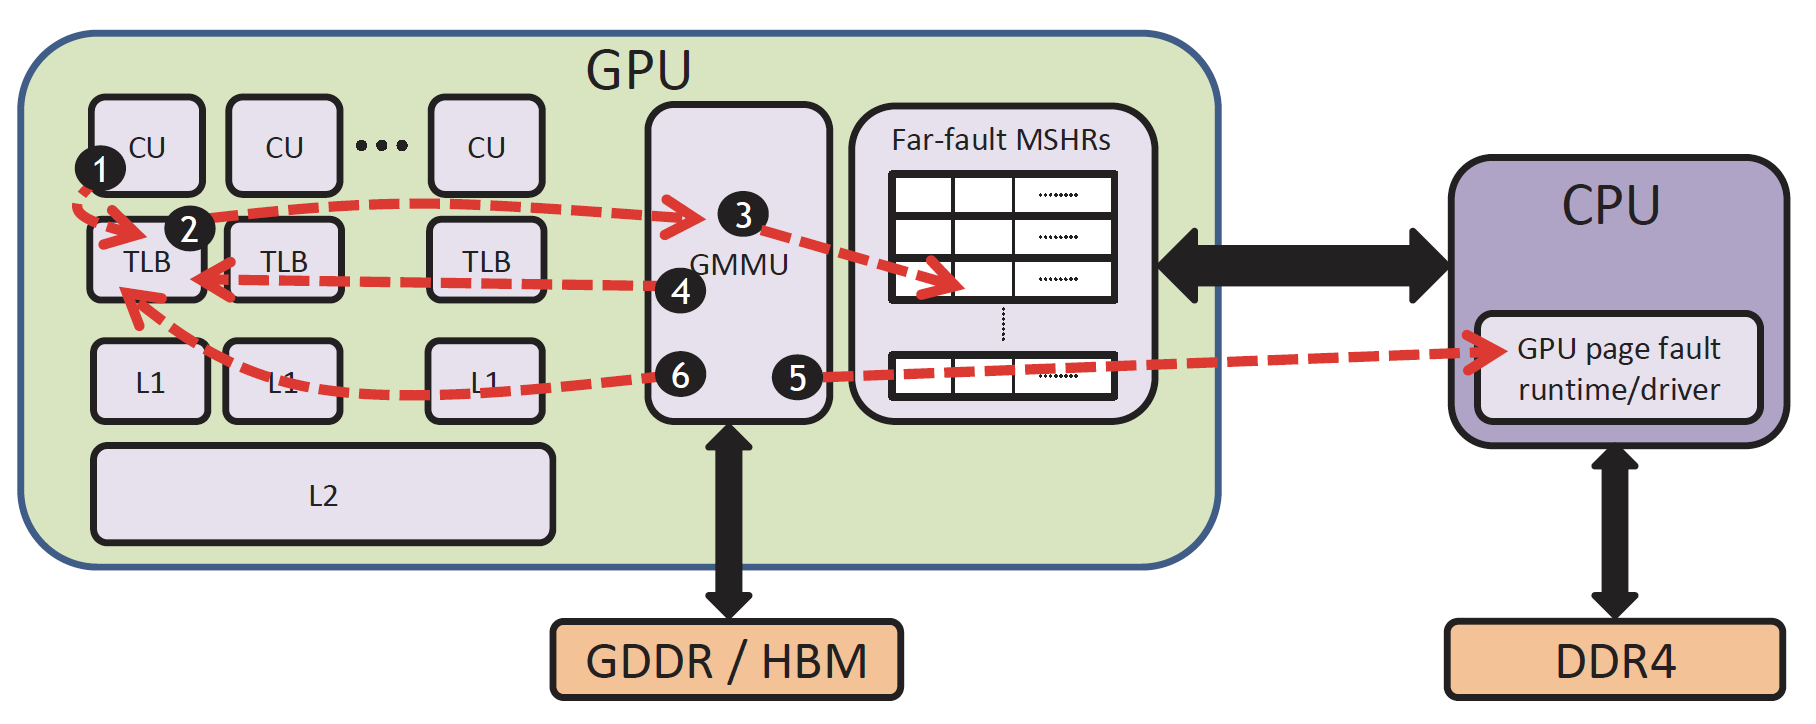
\includegraphics[width=.90\textwidth,keepaspectratio]{figures1/MMU.elf}
      \captionsetup{width=.90\textwidth}
      \caption{Architectural view of GPU MMU and TLBs implementing compute unit (CU) transparent far page faults.
sus}
      \label{fig:mmu}
   \end{figure}
    \subsection{Hardware Prefetchers}
	With UVM, kernel execution stalls at every far-fault for page allocation and data migration from host to device. The total kernel execution time increases dramatically as it includes far-fault handling latency and memory copy time. cudaMemPrefetchAsync, is an asynchronous construct in CUDA 8.0, that allows programmers to specify an address range to migrate in parallel to the kernel execution. Prefetching later referenced pages helps reduce the number of page faults and also ensures overlap between data migration and kernel execution. However, the responsibility of what to prefetch and when to prefetch still belongs to the programmer. Zheng et al are the first to propose programmer-agnostic hardware prefetchers to overlap kernel execution and data migration. They introduced (i) random, (ii) sequential, and (iii) locality-aware hardware prefetchers. Hardware prefetchers take away the burden from the programmer by automatically deciding what and when to prefetch. Following their lead, we have incorporated the following hardware prefetchers in UVMSmart.


\subsubsection{Random Prefetcher}

A random prefetcher prefetches a random 4KB page along with the 4KB page for which the far-fault occurred in the current cycle. The prefetch candidate is selected randomly from the 2MB large page boundary to which the faulty page belongs. This not only helps CUDA workloads with random access pattern, but also selecting from 2MB large page boundary instead of the whole virtual address space helps in cases of locality of memory accesses.

\subsubsection{Sequential-local Prefetcher}

Zheng et al describe their sequential prefetcher as the process of bringing a sequence of 4KB pages from the lowest to the highest order of virtual address irrespective of page access pattern or far-faults. Their locality aware prefetcher migrates consecutive 128 4KB pages (or total 512KB memory chunk) starting from the faulty-page. We propose a different variation called sequential-local hardware prefetcher. Each cudaMallocManaged allocation is logically split into multiple 64KB basic blocks. GMMU upon discovering the pages corresponding to the coalesced memory requests are in-alid in the GPU page table, first calculates the base addresses of the 64KB logical chunks to which these faulty 4KB pages belong. Thus, GMMU identifies these 64KB basic blocks as prefetch candidates. Further, it divides these candidate basic blocks into prefetch groups and page fault groups based on the position of the faulty page in the current basic block and then schedules them for sequential transfers by the PCI-e interconnect. Prefetching 64KB basic blocks ensures contiguous 16 4KB pages local to the current faulty pages. The position of a faulty page can be anywhere within the corresponding 64KB basic block. Further, multiple faulty pages are taken in consideration while choosing a basic block for prefetching and can be grouped within the same 64KB boundary.

\subsubsection{Tree-based Neighborhood Prefetcher}

    \begin{figure}[!htb]
      \centering
      \setlength{\abovecaptionskip}{6pt plus 1pt minus 1pt}
      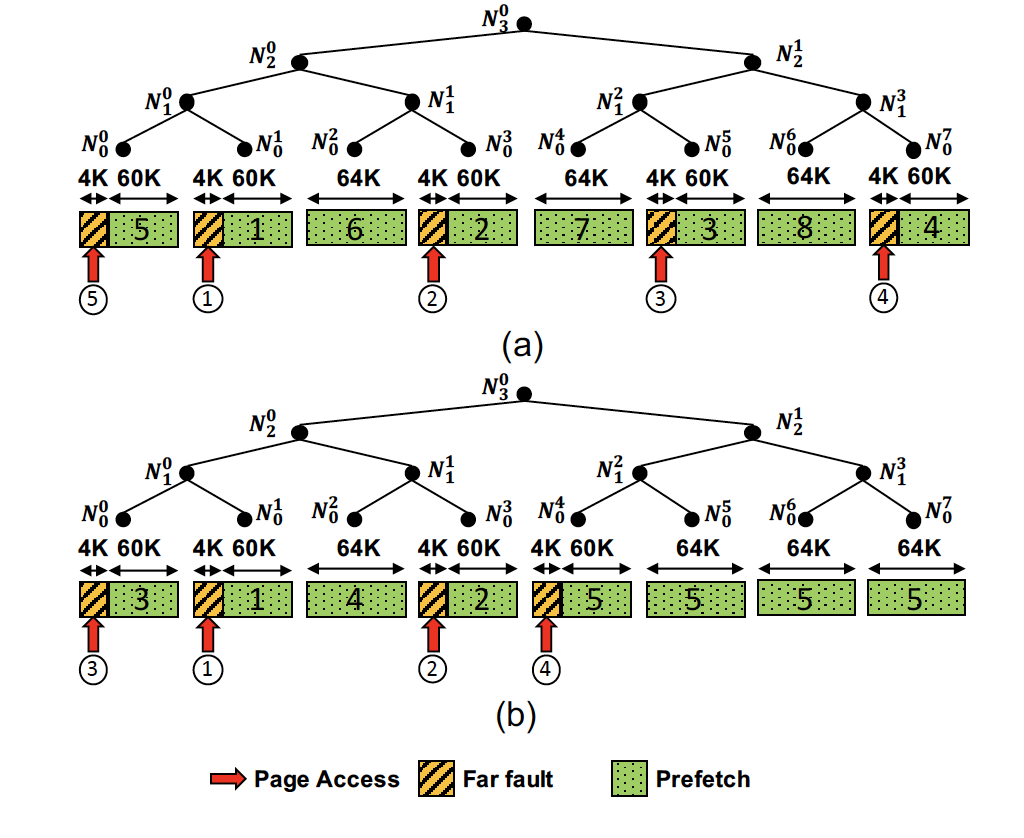
\includegraphics[width=.90\textwidth,keepaspectratio]{figures1/prefetchers.elf}
      \captionsetup{width=.90\textwidth}
      \caption{Demonstration ofTBNp on 512 KB memory chunk for two different page access patterns.}
      \label{fig:prefetchers}
    \end{figure}

The semantics of TBNp demands that every cudaMallocManaged allocation is first logically divided into 2MB large pages. Then, these 2MB large pages are further divided into logical 64KB basic blocks to create a full binary tree  per large page boundary. By the definition of a full binary tree, every node has exactly 2 children nodes. The root node of each binary tree corresponds to the virtual address of a 2MB large page and the leaf-level nodes correspond to the virtual addresses of the 64KB basic blocks. If the user-specified size of an allocation is not a perfect multiple of 2MB, then the remainder size of the allocation breaks the principle of a full binary tree. To address this, the remainder allocation is rounded up to the next $2^i * 64$KB and another full binary tree is created. For example, if the programmer specifies 4MB and 192KB size for a cudaMallocManaged allocation, at the time of allocation, GMMU rounds this size up to 4MB and 256KB. Then two full binary trees for 2MB large pages and one full tree for 256KB are created and maintained by the GMMU transparent to the programmer’s knowledge. This behavior can also be verified by running the micro-benchmarks we have published. 

The maximum memory capacity of a node in the full binary tree can be calculated as $2^h * 64$KB, where h is the height of a node and h = 0 at the leaf level. On every far-fault, the GMMU first identifies the 64KB basic block corresponding to the faulty page being requested. With the understanding that upon migrating, 16 pages in the basic block will be validated in the GPU page table, GMMU then recalculates the to-be valid size of its parent and grand- parent up to the root node of the tree. Here and henceforth, by valid size we mean the size of all valid pages corresponding to the leaf- nodes belonging to a given node. At any point, if GMMU discovers the to-be valid size of a node is strictly greater than 50% of the maximum memory capacity at this level, it tries to balance the valid sizes between the two children of that node. This balancing process is recursively pushed down to the children which have not reached the maximum valid size quota. This balancing act identifies basic blocks for prefetching. This process continues till no more basic blocks at leaf level can be identified as prefetch candidates and the to-be valid size of any non-leaf node including root is not more than 50% of maximum size capacity at its level. 

Prefetching contiguous pages within 2MB boundary tries to ensure allocation of larger contiguous memory and can also help bypass traversing the nested page tables. This helps reduce the time to access memory. For this same reason, researchers introduced the concept of memory defragmentation to swap and coalesce fragmented memory chunks to ensure contiguous physical memory worth of 2MB large page. However, migrating 4KB pages on-demand and then defragmenting the memory space in the runtime has a substantial overhead. Whereas, TBNp is an adaptive scheme where the prefetch size can vary from 64KB to 1MB based on the access pattern and opportunity of prefetching. Thus, it can get close to 2MB large page locality without causing any additional performance overhead. 

TBNp can be demonstrated with the help of two examples in Figure \ref{fig:prefetchers}. Both of these examples explain the semantics on 512KB memory chunk for simplicity. These examples use $N_h^I$ to denote a node in the full binary tree, where $h$ is the height of the node and i is the numeric position of the node in that particular level. We further assume initially all pages in this 512KB allocation are invalid with valid bit not set in the GPU’s page table and thus every first access to a page causes a far-fault. In the first example, for the first four far-faults, GMMU identifies the corresponding basic blocks $N^1_0$ , $N^3_0$ , $N^5_0$ , and $N^7_0$ for migration. In the example, as the first byte of every basic block is accessed, the basic blocks are split into 4KB page-fault groups and 60KB prefetch groups. All memory transfers are serialized in time. After these first four accesses, each of nodes $N^1_0$ , $N^3_0$ , $N^5_0$ , and $N^7_0$ has 64KB valid pages. Then, GMMU traverses the full tree to update the valid page size for all the parent nodes and thus each node at $h = 1$ ($N^1_0$ , $N^1_1$ , $N^2_1$ , and $N^3_1$) has 64KB valid pages. When the fifth access occurs, GMMU discovers that $N^0_1$ and $N^0_2$ will have 128KB and 192KB valid pages respectively. For $N^0_2$, the to-be valid size is greater than 50% of the maximum valid size of 256KB. Hence, the right child $N^1_1$ is identified for prefetching. This decision is then pushed down to the children. This process identifies the basic block $N^2_0$ as a prefetch candidate. Further, GMMU discovers that after prefetching $N^2_0$, $N^0_3$ will have 320KB of valid pages which is more than 50% of the maximum valid size of 512KB. Then, node $N^0_3$ pushes prefetch request to the node $N^1_2$ which in turn pushes it to its children. This process identifies basic blocks $N^4_0$ and $N^6_0$ for further prefetching.

In the second example, the first two far-faults cause migration of basic blocks $N^1_0$ and $N^3_0$. GMMU traverses the tree to update the
valid size of nodes $N^0_1$ and $N^1_1$ as 64KB each. At the third far-fault, as basic block $N^0_0$ is migrated, the estimated valid sizes for nodes $N^0_1$, and $N^0_2$ are updated as 128KB and 192KB respectively. As the valid size of $N^0_2$ is more than 50% of the maximum valid size of 256KB, $N^2_0$ is identified for prefetching. After this point, the $N^0_2$ is fully balanced and both $N^0_2$ and $N^0_3$ have exactly 256KB of valid pages. On fourth access, GMMU discovers that the valid size of $N^0_3$ will be 320KB which is more than 50% of the maximum memory size it can hold. This imbalance causes prefetching of nodes $N^5_0$ , $N^6_0$, and $N^7_0$. Note at this point as GMMU finds four consecutive
basic blocks, it groups them together to take advantage of higher bandwidth. Then, based on the page fault, it splits this 256KB into two transfers: 4KB and 252KB. An interesting point to observe here is that for a full binary tree of 2MB size, TBNp can prefetch at most 1020KB at once in a scenario similar to the second example.
\section{UVM Smart Integration}
    \subsection{Merge Code}
        Table \ref{tab:apis} enumerates the CUDA API calls regarding to UVM currently supported by UVM Smart. These calls are enough to enable the execution of shared virtual memory space programming model. UVM Smart mainly adds on the modeling of far-fault handling latency and PCI-e transfer latency. Based on the Table \ref{tab:pcie}, a function to express PCI-e bandwidth as a function of transfer size is deducted. In the simulator, PCI-e transfer latency is calculated based on this expression.  an additional 100 core cycles for page table walk. The simulator makes simplified assumptions to model TLB and page table. The TLB look up is performed in a single core cycle based on the assumption of fully-associative TLB. A multi-threaded model for page table walk is used and an additional fixed 100 core cycles for page table walk is considered.

    \begin{table}[!htbp]
        \centering
        \setlength{\abovecaptionskip}{6pt plus 1pt minus 1pt}
        \captionsetup{width=.75\textwidth}
        \caption {CUDA API Calls Supported by UVMSmart.}
            \begin{tabular}{|l|l|c|}
                \hline
                \textbf{Transfer Size (KB)} & \textbf{PCI-e Bandwidth (GB/s)} \\
                \hline
                4 & 3.2219 \\
                \hline
                16 & 6.4437 \\ 
                \hline
                64 & 8.4771  \\
                \hline
	        256 & 10.508  \\
                \hline
		1024 & 11.223  \\
                \hline
            \end{tabular}
        \label{tab:pcie}
    \end{table}

    \begin{table}[!htbp]
        \centering
        \setlength{\abovecaptionskip}{6pt plus 1pt minus 1pt}
        \captionsetup{width=.75\textwidth}
        \caption {CUDA API Calls Supported by UVMSmart.}
            \begin{tabular}{|l|c|c|}
                \hline
                CUDACall  \\
                \hline
                \hline
                \texttt{cudaMallocManaged}  \\
                \hline
                \texttt{cudaDeviceSynchronize}  \\
                \hline
                \texttt{cudaMemprefetchAsync}  \\
                \hline
            \end{tabular}
        \label{tab:apis}
    \end{table}
    
The first step in merging UVMSmart into GPGPU-Sim is to understand the difference between them. Since UVMSmart extended GPGPU-Sim v3.2, the major change is a new class, called \texttt{gmmu\_t}, that handles the gpu memory management added to UVMSmart. This class stores necessary information about memory requests from all shader cores that missed in TLB. Then it figures out whether there is page-fault by looking up the page table. If page-fault, it would coalesce faults to the same page and handle these page faults one by one. If hardware prefetched is enabled, it would bring extra pages to GPU memory in the light of prefetching algorithms(Section B.4). And the update from GPGPU-Sim v3.2 to v4.0 has some minor changes, like making simulation cycle count a class variable instead of a global variable. Such minor changes would cause simulation crashes if not noticed and changed properly.

Table \ref{tab:uvm_tests} lists the number of benchmarks from various benchmark suites (Rodinia, Parboil, Lonestar, Parboil, HPC Challenge) that modified to use UVM.

    \begin{table}[!htbp]
        \centering
        \setlength{\abovecaptionskip}{6pt plus 1pt minus 1pt}
        \captionsetup{width=.75\textwidth}
        \caption {UVM Smart benchmarks}
            \begin{tabular}{|l|c|c|}
                \hline
                \textbf{Benchmark} & \textbf{Input} &  \textbf{Output}\\
                \hline
                bfs &  4096 & \\
                \hline
                hotspot & 30 6 40 & \\
                \hline
                pathfinder & 1000 20 5 & \\
                \hline
                backprop & 65536 & \\
                \hline
                srad & 1024 127 .5 4 & \\
                \hline
            \end{tabular}
        \label{tab:uvm_tests}

    \end{table}

 The configuration for the GPGPU Simulator supporting Unified Virtual Memory is shown in Listing \ref{lst:sst_config}.


\lstdefinelanguage{mooCows}
{
  basicstyle={\small\ttfamily},
  columns=flexible,
  tag=[s]{[]},
  tagstyle=\color{dkgreen}\bfseries,
  usekeywordsintag=true
}[html]

\lstset{frame=tb,
  language=mooCows,
  aboveskip=3mm,
  belowskip=3mm,
  showstringspaces=false,
  columns=flexible,
  basicstyle={\small\ttfamily},
  numbers=none,
  numberstyle=\tiny\color{gray},
  breaklines=true,
  breakatwhitespace=true,
  tabsize=3
}

\lstinputlisting[caption=Sample GPGPU-Sim UVM Smart Configuration, label=lst:sst_config]{figures1/config}


    \subsection{Optimize Simulation Performance}
        In Section B.1 and B.2, we mentioned that GPUs may choose to implement page-fault handling by having the GMMU stop the GPU TLB from taking new translation requests until the SW runtime has performed the page migration and GMMU can successfully return a page translation. Under such a scenario, each individual CU could be blocked for thousands of cycles while its page fault is handled, but other non-faulting compute units can continue make progress, enabling some overlap between GPU kernel execution and on-demand memory migration. Alternatively, to enable the CU to continue executing in the presence of a page-fault, the CU TLB and GMMU need to be augmented. Even though UVM Smart choose the latter that enables compute unit execution under page faults, in the worst case, page-fault latency cannot be hidden if all warps are waiting for their page-fault handling requests, especially common at the beginning of kernel execution.

The page-fault latency includes the page-fault handling latency and page migration time. As described in section C.1, the page-fault handling latency is fixed and the page migration time is calculated once the memory transfer size is known, thus the simulator knows in which cycle the pages is ready in GPU memory before the page-fault handling request is sent. This simulator assumption is a opportunity to skip those cycles when all warps are stalled due to page-fault handling.


    \begin{table}[!htbp]
        \centering
        \setlength{\abovecaptionskip}{6pt plus 1pt minus 1pt}
        \captionsetup{width=.75\textwidth}
        \caption {CUDA API Calls Supported by UVMSmart.}
            \begin{tabular}{|l|c|c|}
                \hline
                CUDACall  \\
                \hline
                \hline
                \texttt{cudaMallocManaged}  \\
                \hline
                \texttt{cudaDeviceSynchronize}  \\
                \hline
                \texttt{cudaMemprefetchAsync}  \\
                \hline
            \end{tabular}
        \label{tab:apis}
    \end{table}
    \subsection{Improve TLB performance}
        An important correctness issue of TLB shootdown seems promising to be studied. The GPU MMU design handles TLB flushes similarly to the CPU MMU. Particularly when the register which stored the pointer to the page table is written, the GPU MMU is notified via inter-processor communication and all of the GPU TLBs are flushed. This is a rare event, usually happens between two different kernels. A more common case is when a page-fault occurs and a new page is brought to GPU memory, all TLBs need to be flushed because the MMU does not know which TLB has stale translation infomation.

Mechanisms to reduce the cost of TLB shootdowns on CPUs, and emerging heterogeneous memory systems, have attracted significant attention over the last decade. This is due to the rising cost of TLB shootdowns, especially as core counts continue to scale and heterogeneous memory makes its way into mainstream systems. Previous work by Agarwal et al. have studied on mechanisms to reduce the occurrence of TLB shootdowns on a CPU-GPU system. Reducing the cost for translation coherence on virtualized systems has also been studied.

With UVM Smart simulation framework, it would not be hard to gain the insight of TLB performance. Therefore, we run an experiment in terms of GPU TLB shootdown granularity. We want to justify the positive impact of advanced TLBs. The result shows that the TLB shootdown penalty is not significantly varied among different shootdown granularity.


   \begin{figure}[!htb]
      \centering
      \setlength{\abovecaptionskip}{6pt plus 1pt minus 1pt}
      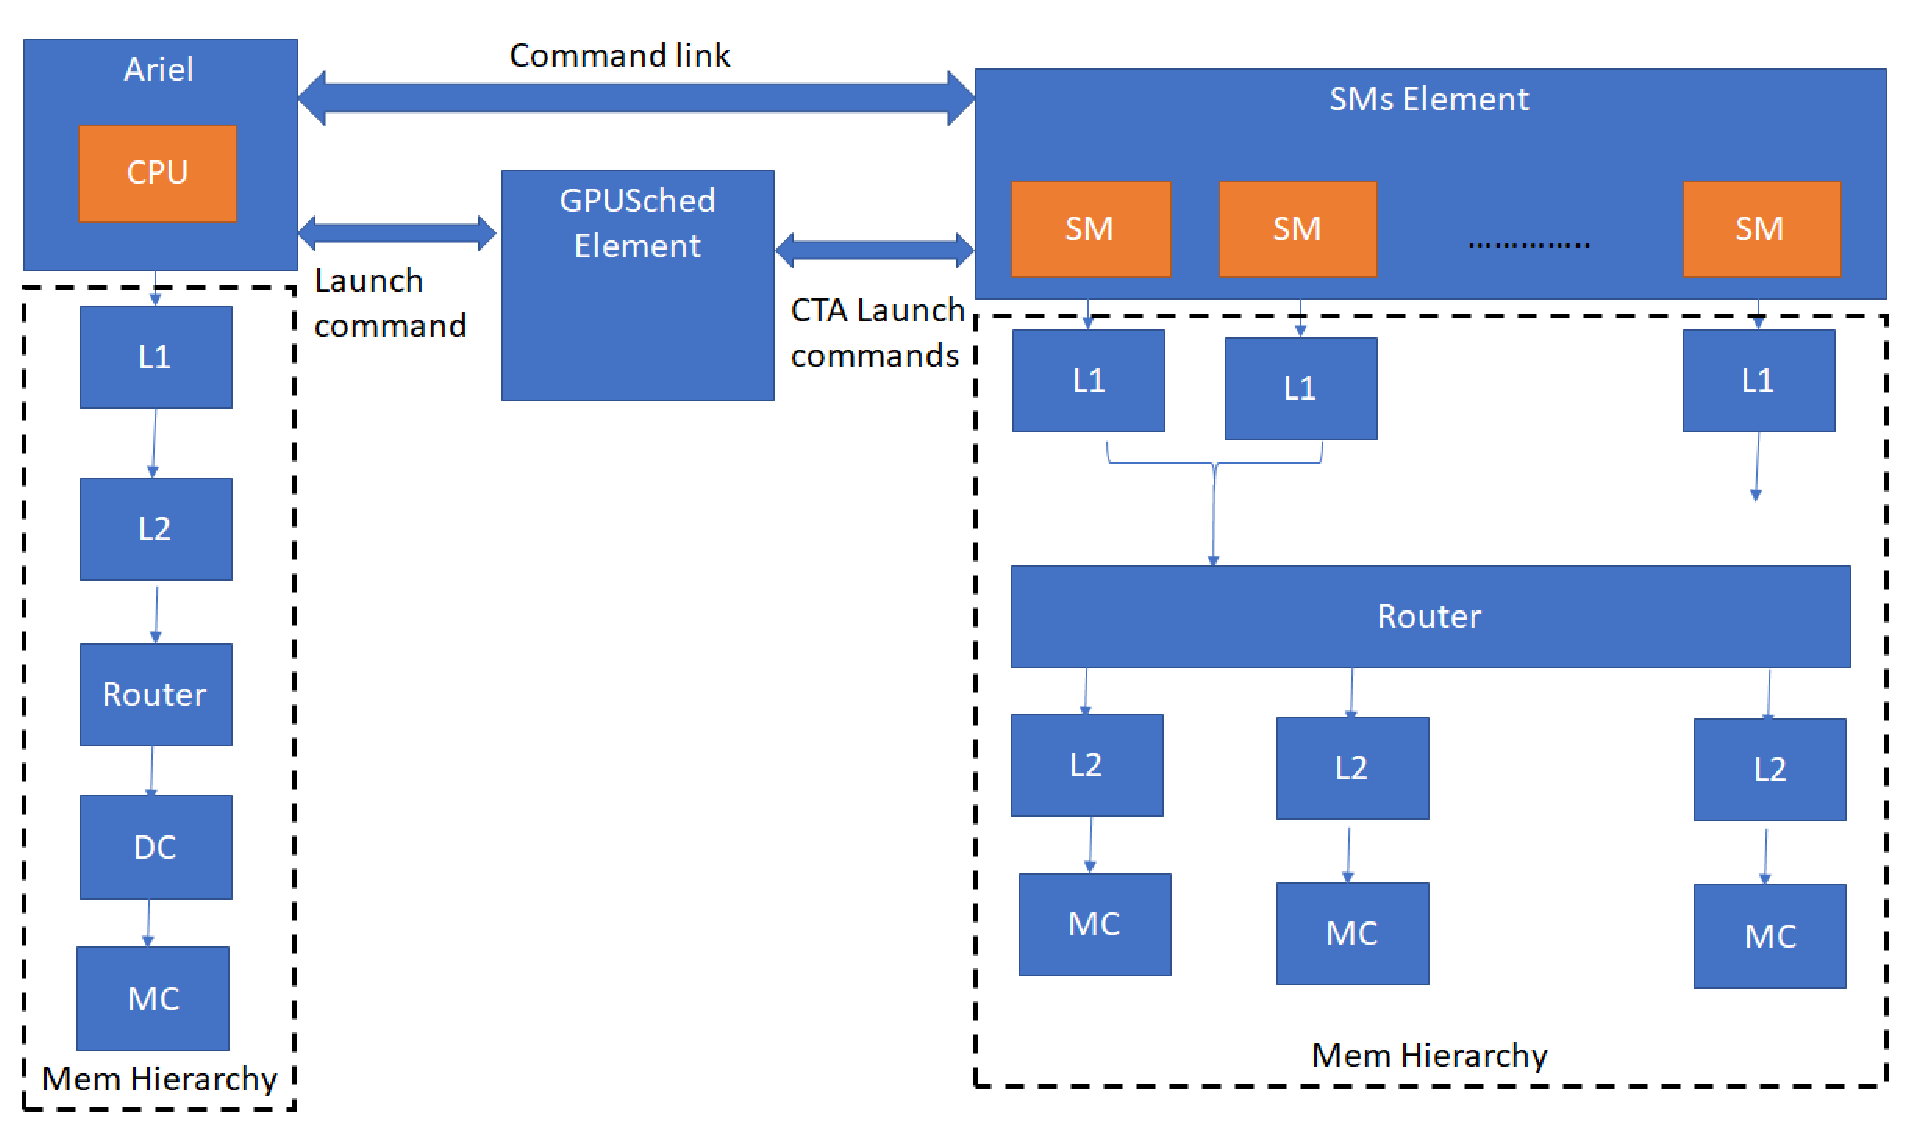
\includegraphics[width=.90\textwidth,keepaspectratio]{figures/3_1.eps}
      \captionsetup{width=.75\textwidth}
      \caption{Timing and memory model for SMs component}
      \label{fig:gpu_mem_model}
   \end{figure}

\section{Evaluation}
    \subsection{Correlation}
        A validation sweep was run using six benchmarks. These
applications were run using UVM Smart model that approximates a Nvidia V100. The simulation parameters are shown in Table
\ref{tab:v100_params}. The overall kernel runtime was compared with the results
of running the six applications through nvprof on Nvidia Tesla V100. Figure \ref{fig:correlation}
shows the total number cycles that each application took on the simulation model
and on the native V100. Note that this is only cycles where a kernel was running
and does not include host execution time. The performance gap mainly comes from prefetching algorithms. The blue cross points represent the result of no prefetcher applied, the yellow represents random prefetched, the black represents the sequential locality prefetcher, and the cyan represents the tree-based neighbor prefetcher. It is very clear that the tree-based neighbor prefetcher has the best correlation, which seems very close to the tree-based hardware prefetcher implemented by NVIDIA CUDA driver.

   \begin{figure}[!htb]
      \centering
      \setlength{\abovecaptionskip}{6pt plus 1pt minus 1pt}
      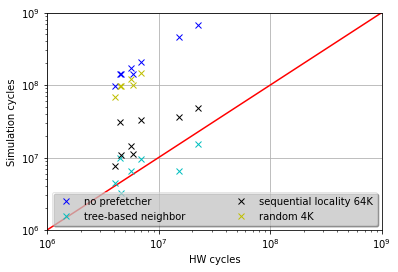
\includegraphics[width=.90\textwidth,keepaspectratio]{figures1/corre.elf}
      \captionsetup{width=.75\textwidth}
      \caption{Correlations between simulator and hardware.}
      \label{fig:correlation}
   \end{figure}


    \begin{table}[!htbp]
      \centering
      \setlength{\belowcaptionskip}{6pt plus 1pt minus 1pt}
      \captionsetup{width=.75\textwidth}
      \caption{CPU/V100 Model Parameters}
      \hspace{1cm}
         \begin{tabular}{|l|c|}
            \hline
            Clock                 & 1312MHz          \\ \hline
            SMs                   & 84               \\ \hline
            L2 Slices             & 32               \\ \hline
            L2 Capactiy           & 192KiB per slice \\ \hline
            HBM Capacity          & 16384MiB         \\ \hline
            HBM Stacks            & 4                \\ \hline
            Crossbar Frequency    & 1200MHz          \\ \hline
            Crossbar Input Ports  & 2                \\ \hline
            Crossbar Output Ports & 1                \\ \hline
         \end{tabular}
      \label{tab:v100_params}
   \end{table}
    \subsection{Kokkos}
        As we stated in C.3, an experiment is designed to justify the positive impact of advanced TLBs. We compared two TLB shootdown granularities - per TLB entry v.s. whole TLB when the GPU page table is updated. The default implementation is to invalidate the whole TLB of every CU. Alternatively, only one TLB entry will be modified with TLB coherence. Although TLB coherence requires additional hardware support, it should have similar behavior with per TLB entry shootdown in terms of TLB hit rate.


As expected, smaller shootdown granularity gives higher hit rate because it keeps as much as valid translation information at any given time. The average hit rate difference is 11%.
However, TLB shootdown granularity has little effect on simulation cycles. This result demonstrates that if there is no significant latency improvement, the GPU barely benefit from TLB coherence model.

    \begin{figure}[!htb]
      \centering
      \setlength{\abovecaptionskip}{6pt plus 1pt minus 1pt}
      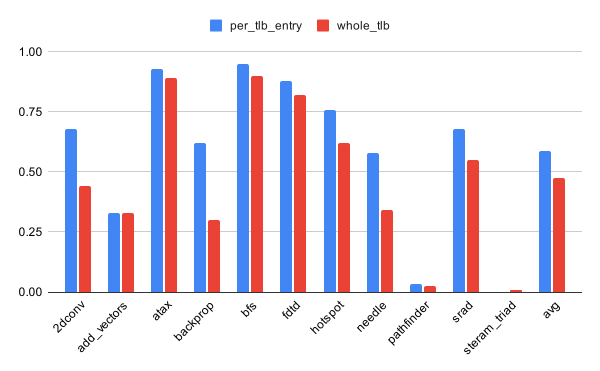
\includegraphics[width=.90\textwidth,keepaspectratio]{figures1/tlb_hit_rate.elf}
      \captionsetup{width=.75\textwidth}
      \caption{TLB hit rate for per TLB entry shootdown and whole TLB shootdown.}
      \label{fig:tlb_hr}
   \end{figure}

   \begin{figure}[!htb]
      \centering
      \setlength{\abovecaptionskip}{6pt plus 1pt minus 1pt}
      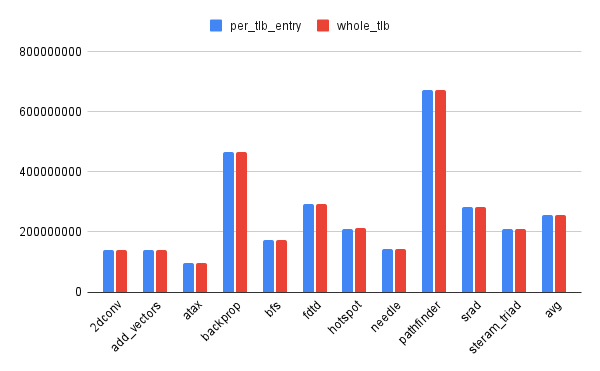
\includegraphics[width=.90\textwidth,keepaspectratio]{figures1/tlb_cycles.elf}
      \captionsetup{width=.75\textwidth}
      \caption{Simulation cycles for per TLB entry shootdown and whole TLB shootdown.}
      \label{fig:tlb_cycles}
   \end{figure}

    \subsection{Lulesh}
        A parameter sweep was performed using LULESH, described in Section
\ref{sec:lulesh}. The device clock was varied from 500MHz to 1312MHz to 1800MHz.
The memory clock was varied from 877MHz to 1200MHz to 1600MHz. Figure
\ref{fig:lulesh_sweep} shows the results, where lower runtime time is better.


As expected, changing the frequency of the backing store has little effect on
LULESH for this problem size because it is not memory bandwidth bound. The most
improvement is seen at the low device clock frequency, but at this frequency
the speedup is still small at 1.04x.
However, increasing the frequency of the SMs does improve the
performance noticeably. Going from 500MHz to 1312MHz shows a 2.5x speedup; going
from 1312MHz to 1800MHz shows a further 1.3x speedup.

Although this was a small study, one can imagine being able to run a more
complete parameter sweep over any of the Balar parameters.

   \begin{figure}[!htb]
      \centering
      \setlength{\abovecaptionskip}{6pt plus 1pt minus 1pt}
      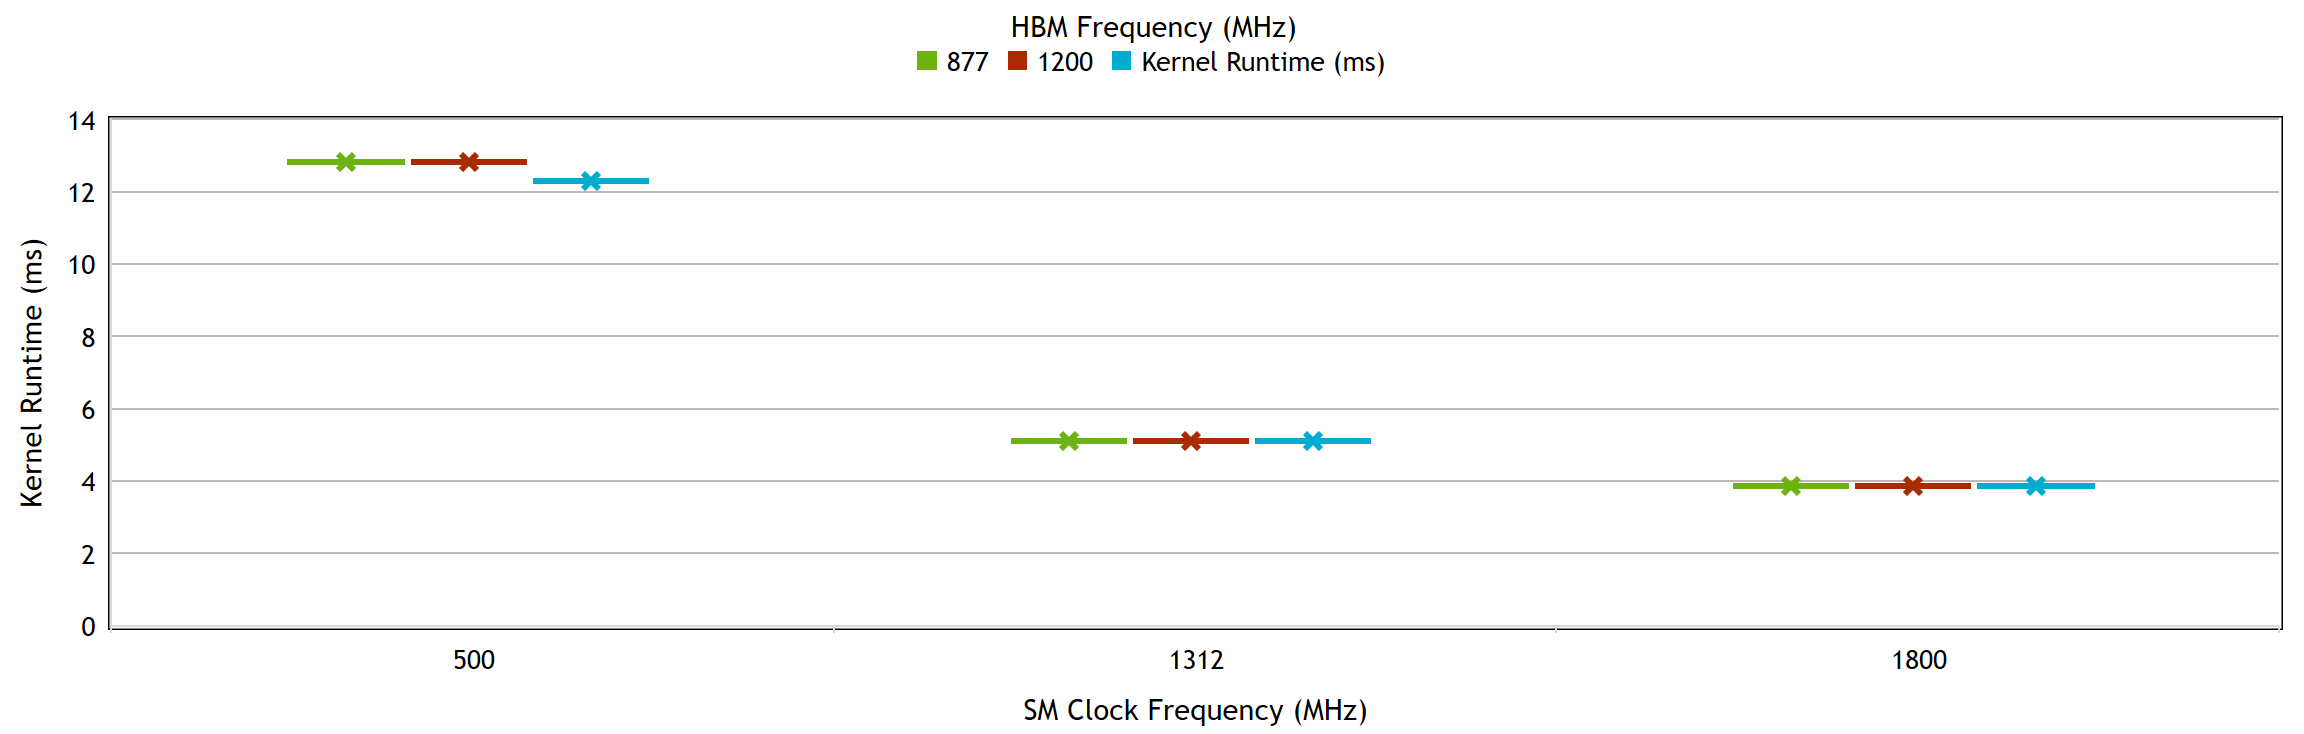
\includegraphics[width=.98\textwidth,keepaspectratio]{figures/lulesh_sweep.png}
      \captionsetup{format=hang, justification=centering, width=.75\textwidth}
      \caption[GPU Parameter Sweep Using LULESH]{GPU Parameter Sweep Using LULESH\\(Baseline was 1312MHz/877MHz)}
      \label{fig:lulesh_sweep}
   \end{figure}


% Design space exploration is not the only use case for this integration. One of
% the more novel features of SST is the ability to obtain periodic statistic dumps
% for all of the currently loaded components. This presents enormous opportunities
% for system designers and application developers. Modern performance profiling
% tools can only provide users with, relatively, coarse-grain details from
% performance counters. SST can provide statistics for any component in the model
% at a time granularity defined by the user. The plots in the figures below are
% all at a 2us granularity. Imagine being able to query that information on any
% time scale for any of the ~20k component statistics in this model! Figure
% \ref{fig:time_sweep} shows an example of this with the host activity plotted in
% \ref{fig:host_cycles} and the GPU crossbar activity plotted in
% \ref{fig:crossbar_activity} (used here as a stand-in for GPU activity).
%
% Kernel launches are asynchronous with the host unless explicitly declared otherwise.
% Even memory copies from the host to the device are asynchronous in this model -- the
% scheduling unit queues all work from a given stream and can guarantee correctness.
%
%    \begin{figure}[!htb]
%       \centering
%       \setlength{\abovecaptionskip}{6pt plus 1pt minus 1pt}
%       \subfigure[Host Cycles]{
%          \label{fig:host_cycles}
%          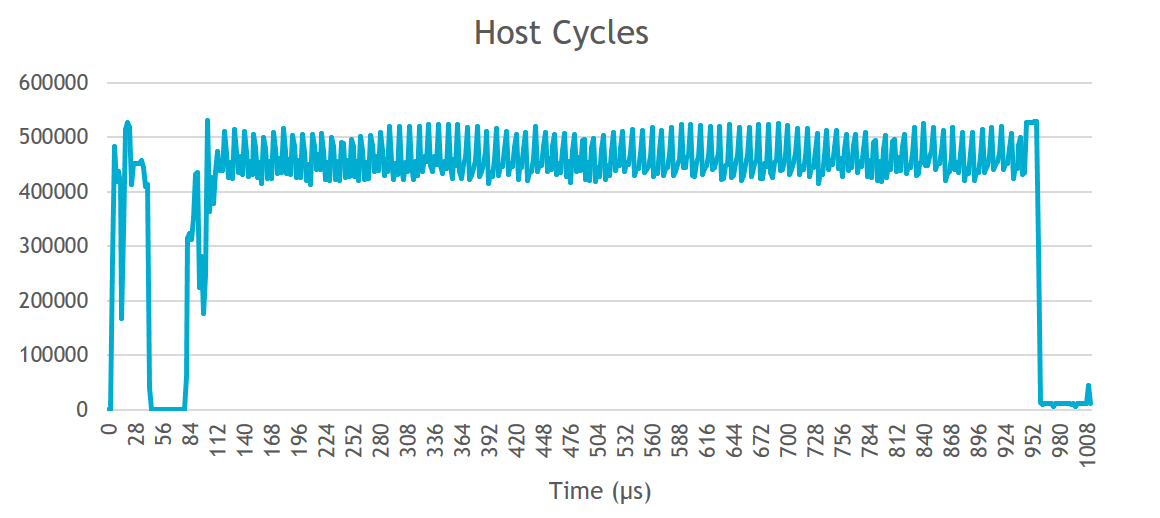
\includegraphics[width=.48\textwidth,height=4cm]{figures/host_cycles.png}
%       }
%       \subfigure[Device Crossbar Activity]{
%          \label{fig:crossbar_activity}
%          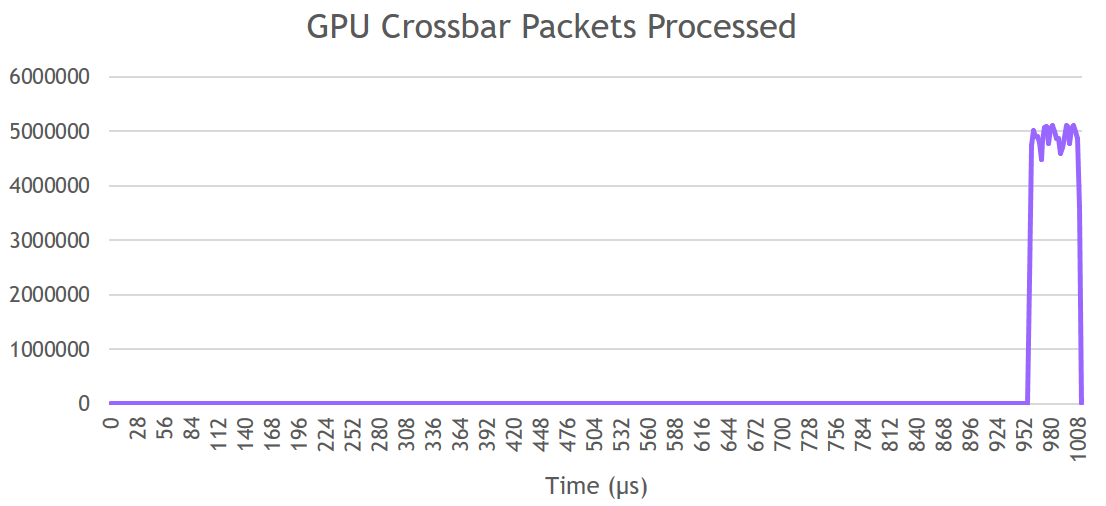
\includegraphics[width=.48\textwidth,height=4cm]{figures/crossbar_packets.png}
%       }
%       \caption{Full caption.}
%       \label{fig:time_sweep}
%    \end{figure}

    \subsection{Parallel Simulation Performance}
        \fixme{@Mengchi - put the new performance data and discussion in here. Make sure
to run it through Grammarly and I will vett it too.}


%To evaluate the performance correlation of our GPU-SST model, versus both real
hardware and the existing GPGPU-Sim memory system implementation an execution
time correlation is done on the vectorAdd benchmark from the CUDA SDK. Figure
\ref{fig:titanv_result} shows the results of this timing analysis. The most
accurate GPGPU-Sim timing model is reasonably accurate (within 25\% of the
hardware results), however GPU-SST is much closer to real hardware, showing
just and 8\% deviation from a silicon Nvidia Titan V card.


   \begin{figure}[!htb]
      \centering
      \setlength{\abovecaptionskip}{6pt plus 1pt minus 1pt}
      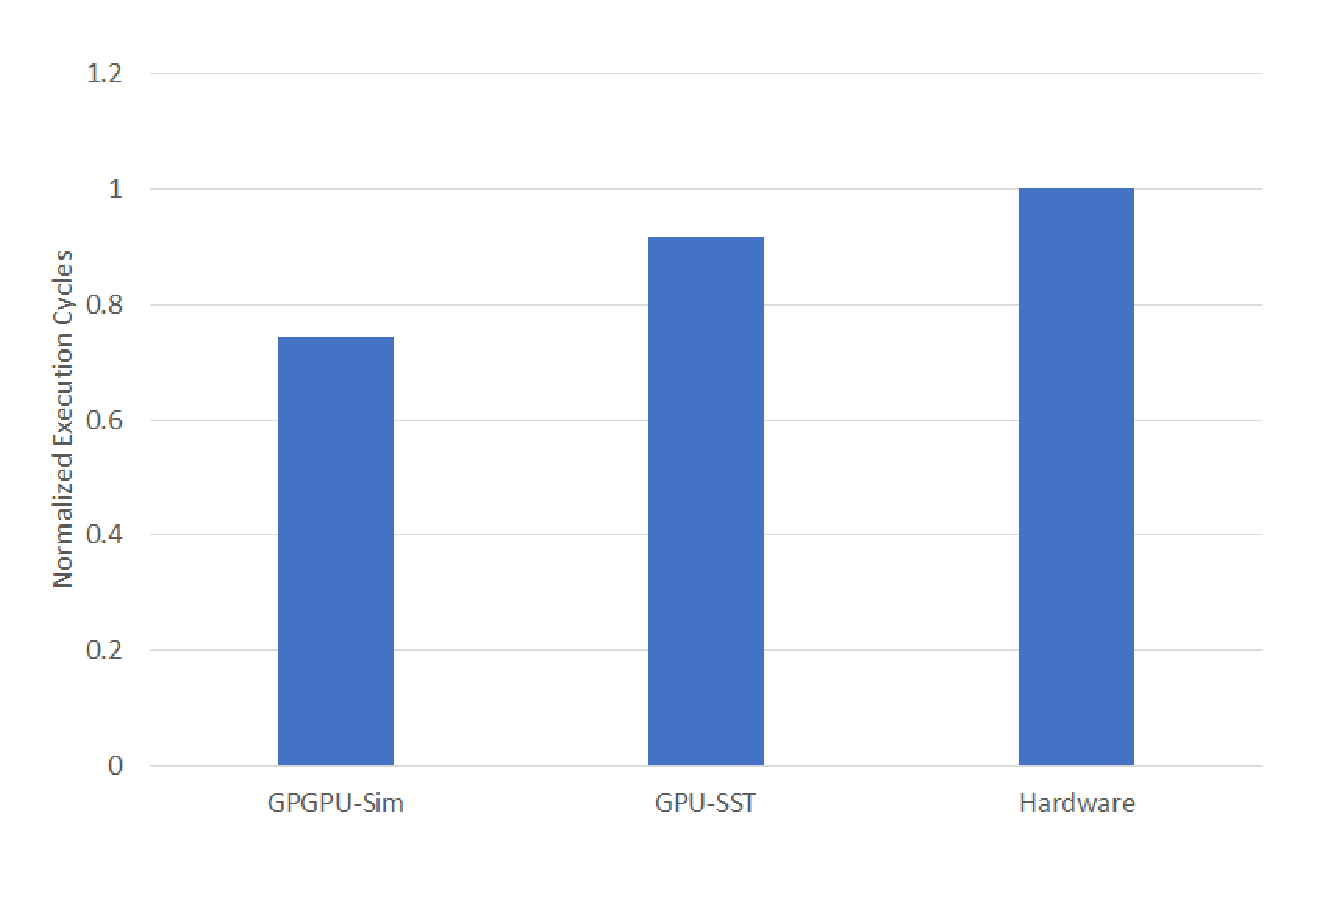
\includegraphics[width=.50\textwidth,keepaspectratio]{figures/4_1.eps}
      \captionsetup{width=.90\textwidth}
      \caption{Normalized execution time for 160k element vector addition kernel -- \\
               SST-GPU is within 8\% of the silicon of the Titan V}
      \label{fig:titanv_result}
   \end{figure}

\section{Conclusion}
%    This report described the final integration of the SST-GPU project.
Functional validation against the Kokkos Kernels unit tests shows that the GPU
component can successfully run more than XX\% of the tests with a path to reach
a coverage of greater than XX\%. Correlation with the Waterman V100 testbed is
excellent, showing XX\% error in the runtime for the applications considered.
The final phase of the project has involved parallelizing the scheduler and
groups of SMs, dubbed {\em SM Groups}, using multi-threaded.
Initial performance results demonstrate good scalability
using default scheduling policies with additional opportunities to improve
parallel scheduling performance.


\clearpage
\section*{Acknowledgment}
We would like to thank Gwen Voskuilen for her help with memHierarchy and
recommendations on debugging problems with the NIC and interconnect. We would
also like to thank Arun Rodrigues and Scott Hemmert for their support and help
in defining the scope of the project.



\clearpage

\bibliographystyle{plain}
%\bibliography{sst-gpgpu_perf_SAND/sst_gpgpu_perf_SAND}

\end{document}
